The academic discipline of CFD (Computational Fluid Dynamics) emerged in the 1970s as alternative to the experimental and the theoretical approach for the prediction of flows. It relies on the physical modeling of a flow as mathematical problem which is then solved numerical. Nevertheless compared to computer aided engineering fields it lagged behind for a long time due to the tremendous complexity of the underlying models for the description of fluid flows, which should be at the same time economical and physical sufficient correct. Although it comes with huge hardware costs, especially for the LES (Large Eddy Simulation), it is usually still more economical than an experimental facility and comes with various advantages like the capability of the investigation of very large systems, or systems under hazardous conditions.

The analysis and prediction of turbulent flows is a critical factor for the comprehension of natural and technical flow processes. This basis is necessary for the improvement of objects surrounded by a flow like aircraft.

The LES is a subdomain of the CFD and features dedicated filters which reject the smaller eddies and let the larger ones pass. This is done prior to the computation and the smaller eddies are represented by turbulence models. The LES is usually more effort to implement and wrong choices of the models often leads to strong deviations of the results from the actual flow.

This chapter covers the basics of turbulent flows before it deals with the technical principles of LES and heat transfer.

\section{Basics of turbulent flows}
Turbulences appear in a great range of shapes and sizes and independent of their complexity, all flows become unstable above a certain Reynolds number. While flows are usually laminar at low Reynolds numbers they become more and more turbulent, when it increases. This specific value when the flow turns over from laminar to chaotic is called critical Reynolds number.

Turbulences have always three-dimensional spacial character, even if the velocities and pressure vary just in one or two dimensions. The typical signs of turbulence are the so-called turbulent eddies which are basically rotational flow structures as they can be seen in fig \ref{fig:example}. There eddies come with a wide range of various length- and time scales. Due to this rotational flow fields, particles which are initially separated by long distances can be brought together quickly, which leads to a high efficiency in terms of heat, mass and momentum exchange.

Although turbulent flows are highly chaotic and almost impossible to predict over longer periods of time, the characteristic lenghts of the large eddies are proportional to the considered flow problem. An important term which has to be considered in this context is the energy cascade. In a typical turbulent flow kinetic energy is handed down from the large scale eddies, which are by far the most energetic ones, to the smaller ones. Figure \ref{fig:cascade} shows the spectral energy of eddies dependent on their size. Obviously the smaller eddies hold by far the least energy. The large eddies get their energy from the mean flow and break up in the smaller scales. The Reynolds number of the smaller scales equals one, which means that the inertia and the viscous effects are of equal strength. All the work they perform is against the viscous stresses and therefore all the energy they hold dissipates into internal thermal energy.

\begin{figure}[h]
\centering
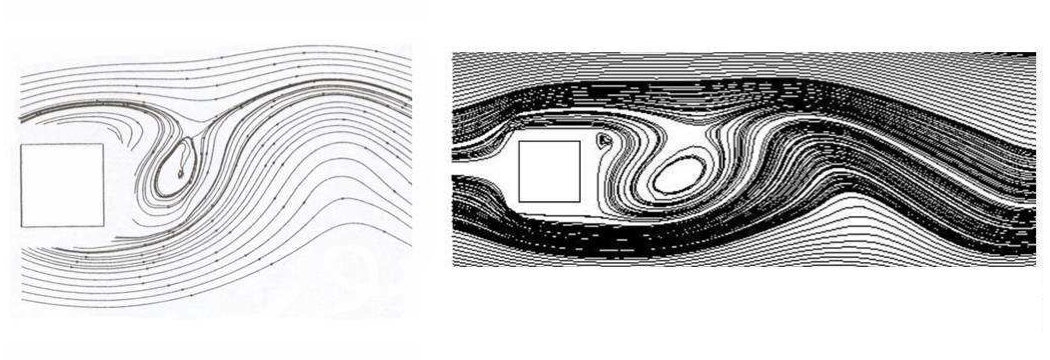
\includegraphics[scale=0.5]{eddies_example.png}
\caption{Experimental and numerical streamlines}
\label{fig:example}
\end{figure}

\begin{figure}[h]
\centering
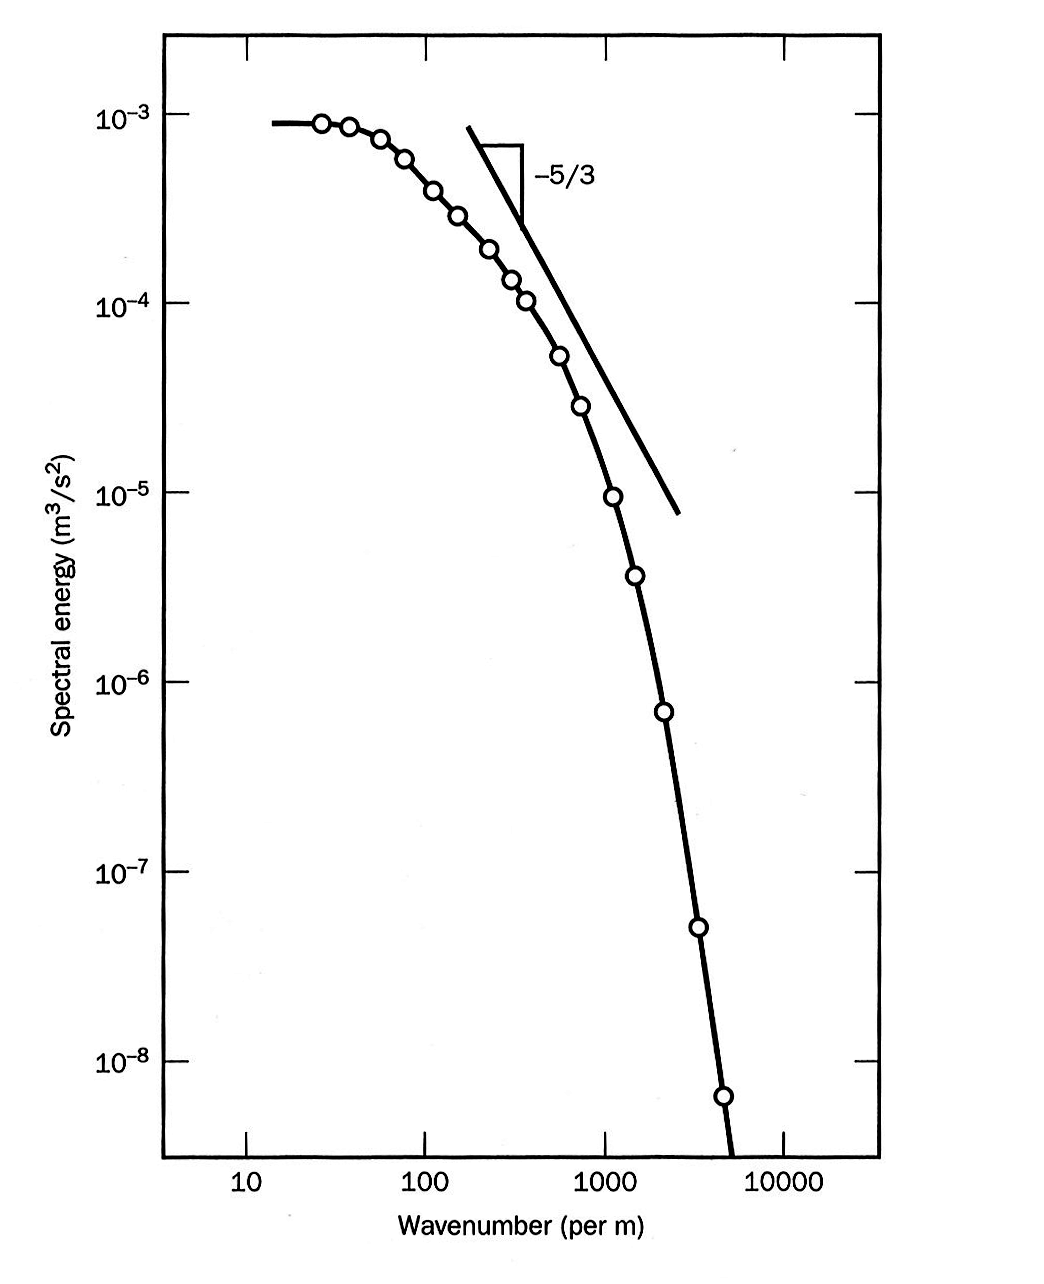
\includegraphics{energy_cascade.png}
\caption{Energy spectrum of turbulence of different scales}
\label{fig:cascade}
\end{figure}

\section{CFD attempts to deal with turbulence}
In CFD there are different ways in order to deal with turbulent flows. All natural flows are more or less turbulent, but in the calculation of flows the turbulences are usually only resolved to a certain degree or omitted altogether. Methods for calculation of flows can be organized according to their turbulence resolving capability.

The so called RANS (Reynolds Averaged Navier-Stokes) equations are the most common and wide-spread approach in order to deal with any flow prediction.
This method yields time averaged properties of the flow like mean velocities, mean pressures, mean stresses, etc. For many technical flow investigation this is enough and therefore this simulation type has been the method of choice for CFD calculations for the past decades. Other advantages are the modest demand on ressources and that two dimmensional calculations are sufficient.
The RANS equations for incompressible flow lead to six additional stresses, known as the Reynolds stresses. This stresses are unknown and for computing turbulent flows they need to be predicted by dedicated turblence models like the k-e model.

The LES (Large Eddy Simulation) represents a sort of compromise between RANS equations and DNS (Direct Numerical Simulation). It has high demands on storage and CPU performance sine unsteady flows need to be computed. Nevertheless, due to the fast improvement of hardware, this method becomes more and more applicable, even for more complex flow problems. As the title suggest this project concentrates mostly on this kind of simulation and therfore it will be discussed in more detail in the following.

With DNS (Direct Numerical Simulation) all scales of turblence are simulated numerical. Therfore a three dimensional is needed which is at least as fine as the the smalest scale eddy. Additionally the timestep needs to be small enough to resolve even the fastest flunctuation. This leads to a tremendous demand of ressources and mesh quality and therefore it is nowadays only performed for academic researches on rather small and simple geometries.

There exist also a lot of sub-forms and mixtures of various approaches, like DES (Detached Eddy Simulation), VLES (Very Large Eddy Simulation), etc., but to mention them would go beyond the scope of this report.

For the project the RANS and the LES simulation have been applied. This chapter is dedicated to introduce the reader to some crucial basics of LES. Therefore it will cover the terms fine structure model, turbulence model and wall function. Due to the numberous different models, equations and the like, each subchapter will deal only with the stuff used for this particual project.

-LES vereinigt elemente aus sehr unterschiedlichen bereichen, insbesondere physik, numerik und turbulenzmodellierung.
\section{Basic idea of Large Eddy Simulation}
Although there have been huge efforts for developing turbulence models since the early days of CFD, a model suitable for a wide range of practial applications and offering convincing results does still not exist. This is due to the very different properties of the different scales of eddies. The smaller eddies are almost isotropic and show universial behaviour while the larger ones interact with and extract energie from the main flow. Their behaviour is heavily dependent on the used geometry and the boundary conditions.
The big advantage of LES is that the larger eddies are computed with a time dependent simulation, while the smaller scales are still represtented by models. However, since the smaller scales are breakdown products of the larger one and represent just a small amount of the overall energy, they are easier to model. With Reynolds-averaged equations on the other hand \emph{all} scales need to be represented by a single turbulence model, which proves especially for the larger eddies inaccurate.

The classification of \emph{small} and \emph{large} eddies is done with dedicated filter functions, which take a \emph{cutoff} width as input parameter. When applied the filter function destroy all the information related to the eddies which are beyond this scale, while the rest remains untouched and gets computated. To describe this association the terms GS (grid scale) and SGS (sub-grid scale) are used. When the smaller ones are left out, also their effect on the flow is omitted. This effect is known as SGS stresses and have to be described by means of so-called SGS models, which are basically turbulence models.

The finer the applied filter is, the more eddies are modelled numericaly and therfore the FS model can be simpler while leading to a similar accurate solution. If the filter becomes, theoretically, indefinitely small the LES passes into a DES. The other margin case would be a very [rau] filter which allows only the most energized eddies. This kind of simulation is known as VLES (Very Large Eddy Simulation).

This circumstances offer two possible options in order to improve the simulation. There can be improved either the FS model or the used grid. In most cases an improvement of the FS model is the option of choice, since a refinement of the grid leads to a much higher demand in terms of resources and comes with no warranty to provide a more accurate solution. However a LES is also highly dependend on the preceding inlet circumstances as well as the wall functions.

\section{Turbulence models}
A majority of the scientific research concerning LES is dedicated to the developement of the so called fine structure modells. They are used to represent the impact SGS symbolically by dissipating as much energy as it would be the case with a DNS modell of the same problem. Most of the fine structure modells used today are deterministic. Therefore the FS (Fine Structure) model is dependend of the velocity field and yields exactly on solution.
\subsection{$k-\varepsilon$ turbulence model}
The $k-\varepsilon$  models are the most frequently used and best prooved model for RANS turbulence. The reason for their popularity is their convincing performance in confinded flow, which is usually the case in industrial application. For these simulations the k-ε model offers a good compromise between accuracy and robustness. In contrast to its excellent performance for many industrially relevant flows it shows some major weaknesses when it comes to unconfined or rotating flows.

The standard $k-\varepsilon$ model presumes an isotropic turbulent viscosity and adds two extra transport equations, one for the $k$ and one for the $\varepsilon$, which need to be solved alongside the RANS flow equations.
The first transported variable $k$ stands for the turbulent kinetic energy and determines the kinetic energie in the turbulence.
The $\varepsilon$ term is responsible for the dissipation and of the dimensions m\textsuperscript{2}/s\textsuperscript{3}. It is of greate importance, especially when it comes to investigation of turbulence dynamics, and roughly of the same order of magnitude as the production term.
\begin{quote}
``The rate of dissipation is per unit volume (VI) is normally written as the product of the density $\rho$ and the rate of dissipation of turbulent kinetic energy per unit mass $\varepsilon$, so
\begin{equation}
\varepsilon = 2 \nu \bar{s^{\prime}_{ij} s^{\prime}_{ij}}
\end{equation}
"
\end{quote}
With $k$ and $\varepsilon$ the the velocity scale $\vartheta$ and the length scale $l$ can be defined as $\vartheta = k^{1/2}$ and $l = k^{3/2}/\varepsilon$. Through this identity the eddy viscosity can be obtained by
\begin{equation}
\mu_t = C \rho \vartheta l = \rho C_{\mu} \frac{k^2}{\varepsilon}
\end{equation}
where $C_{\mu}$ is a dimensionless constant. The additional equations for $k$ and $\varepsilon$ are then:
\begin{equation}
\frac{\partial(\rho k)}{\partial t} + div(\rho k U) = div \left[ \frac{\mu_t}{\sigma_k} grad k \right] + 2 \mu_t S_{ij} S_{ij} - \rho \varepsilon
\end{equation}
\begin{equation}
\frac{\partial(\varepsilon k)}{\partial t} + div(\rho \varepsilon U) = div \left[ \frac{\mu_t}{\sigma_{\varepsilon}} grad \varepsilon \right] + C_{1\varepsilon} \frac{\varepsilon}{k} 2 \mu_t S_{ij} S_{ij} - C_{2\varepsilon} \rho \frac{\varepsilon^2}{k}
\end{equation}
The left side of the equation deals with the rate of change of $k$ or $\epsilon$ plus the transport of by convection, while the right side features the transport by diffusion plus the rate of production minus the rate of destruction of the values $k$ and $\epsilon$.
$C_{\mu}$, $\sigma_k$, $\sigma_{\epsilon}$, $C_{1\epsilon}$ and $C_{2\epsilon}$ are constants with given values for the standard $k-\epsilon$ model and are applicable for a wide range of turbulent flows.

\subsection{Smagorinsky-Lilly SGS model}
The Smagorinsky-Lilly SGS model bases on the assumption that the turbulent stresses are proportional to the mean rate of strain. This approach requires the changes in the flow direction to be slow in order to balance the production and dissipation of turbulence. Furthermore the turbulence structures should be isotropic.
\begin{quote}
``Thus, in Smagorinsky's SGS model the local SGS stresses $R_{ij}$ are taken to be proportional to the local rate of strain of the resolved flow $\bar{S_{ij}} = \frac{1}{2}(\partial \bar{u_i}/\partial x_j + \partial \bar{u_j}/\partial x_i)$:''
\end{quote}
This leads to the equation
\begin{equation}
R_{ij} = -2 \mu_{SGS} \bar{S_{ij}} + \frac{1}{3} R_{ij} \delta{ij} = -\mu_{SGS} \left( \frac{\partial \bar{u_i}}{\partial x_j} + \frac{\partial \bar{u_j}}{\partial x_i} \right) + \frac{1}{3} R_{ii} \delta{ij}.
\end{equation}
The additional term on the right hand side of the equation is responsible that the formula yields the correct results for the normal stresses $\tau_{xx}$, $\tau_{yy}$ and $\tau{zz}$. Due to the deffinition of the Kronecker symbol this term becomes zero for any other stresses. The constant which determines the relation between local stresses and local rate of strain is the dymamic SGS viscosity $\mu_{SGS}$.
The Smagorinsky-Lilly model bases on Prandtl's mixing length model, which comes with the assumption that the kinematic turbulent viscosity $\nu_t$ can be expressed through the velocity scale $\vartheta$ and the turbulent length scale $l$ by
\begin{equation}
\nu_t = C \vartheta l .
\end{equation}
Here $C$ is a dimensionless constant of proportionality. The dynamic viscosity $\mu_{SGS}$ can then simply be obtained by $\mu_{SGS} = \nu{SGS} \rho$. For the lengh scale the cutoff width $\Delta$, used for the filter, is the logic choice.
\begin{quote}
``As in the mixing length model, the velocity scale is expressed as the product of the length scale $\Delta$ and the average strain rate of the resolved flow $\Delta \times |\bar{S}|$, where $|\bar{S}| = \sqrt{2 \bar{S_{ij}} \bar{S_{ij}}}$.''
\end{quote}
Hence the dynamic SGS viscosity can be taken as
\begin{equation}
\mu_{SGS} = \rho (C_{SGS} \Delta)^2 |\bar{S}| = \rho(C_{SGS} \Delta)^2 sqrt{2 \bar{S_{ij}} \bar{S_{ij}}}
\end{equation}
where $C_{SGS}$ is a constant. According to various studies values between 0.1 and 0.24 proved to be appropriate, but occasionally this paramter needs adjustment in order to provide reasonable results.
\section{Heat transfer}
Heat is a special form of energy and is stored in the chaotic movement of atomes and molecules. In a non adiabat system it is the amount of energy which resigns over the border if a temperature gradient is prevailing. The transition of the heat over the system borders is therefore called heat flux and runs always in the direction of the lower temperature.

Basically there are three different ways how heat can be transfered from one system to another. In practical application they usually appear combined but for computation they can be dealt with individually. Each of them will be discussed in the following.
\subsection{Mecanisms of heat transfer}
With conduction, heat gets transfered between particles in immediate viscinity. It occurs with adjacent molecules of solids or steady fluids. If no counteracting processes are pressent the temperature difference becomes sooner or later zero. The heat transfer through a solid wall can be described by means of \emph{Fourier's law}:
\begin{equation}
Q = \frac{\lambda}{\delta} A \Delta t \tau
\end{equation}
The heat conductivity $\lambda$ is a material property and dependent from the temperature. $\delta$ is the thickness of the wall and $\tau$ the duration.

Between moving fluids proceedes the so-called convection. This form of heat transfer is the dominant one in liquids and gases. It occurs in two different forms. Frist, \emph{free convection}, if the flow is caused by the heat transfer itself, which would for example be the case if air flows by a heating device. Sencondly, \emph{forced convection} if the movement is caused by device like a pump of a fan. This would be the case with cooling an engine. 

The last form of heat transfer is by radiation. Radiation is the transmission of energy by means of waves. It can prodeed through different material, altough no material is required for it is also capable of spreading through space. Physically, the internal energy of the radiating system is converted into multiple tiny energies, which are then emited. The movement and location of the single photones cannot be determined, but only the behavior of many photones can be described by means of an electromagnetic wave. Usually the radiation if named after its way of creation, like γ-, or X-radiation. 
The specific radiance M of a body is given by
\begin{equation}
M = \varepsilon \sigma T^4
\end{equation},
where $\varepsilon$ is the emission coefficient and can be taken from dedicated tables.
\subsection{Wall heat flux in Ansys CFX}
The most important property which will be investigated within this project is the wall heat flux. In Ansys CFX this variable represents the total heat flux into the domain, which consists of convective and radiative participations.

The heat flux at a wall boundary is specified by a heat transfer coefficient hc, which is obtained from the equation
\begin{equation}
q_w = h_c (T_0 - T_{\omega} ) = q_{rad} + q_{cond}
\end{equation}
where $T_0$ is the external boundary temperature and $T_{\omega}$ is the temperature at the wall, which is provided explicitly in this project. Figure \ref{fig:ht_in_cfx} pictures how the heat transfer is modelled in Ansys CFX.
\begin{figure}[h]
\centering
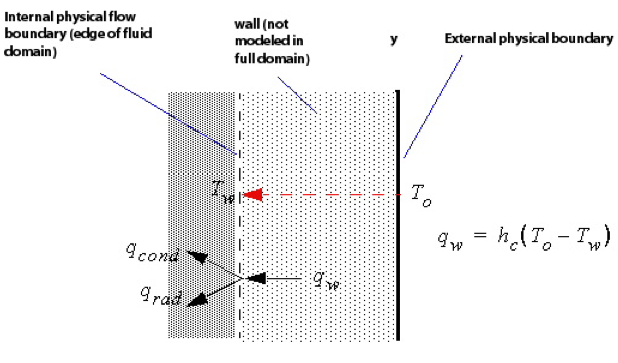
\includegraphics[scale=0.5]{screenshot-heat_transfer_in_cfx.png}
\caption{Heat transfer model in Ansys CFX}
\label{fig:ht_in_cfx}
\end{figure}
\section{Similitude of heat transfer}
It is impossible to determine the heat transfer for every technical problem experimentally. Furtuanatelly it is possible to transfer existing results to physically simiar objects from which the heat transfer coefficient can then be obtained.

The originator of this similitude theorem is Wilhelm Nußelt. The Nußelt number, which is a form of the differential equation of the heat transfer, but with dimensionless parameters, is named after him. It is the dimensionless form of the heat transfer coefficient.
\begin{equation}
Nu = \frac{\alpha l}{\lambda}
\end{equation}
Once the Nußelt number of a specific problem is known the heat transfer coefficient alpha can be easyly calculated. The Nußelt number itself is dependent from other dimensionless number which describe flow- and heat transfer processes.
The most important ones are the Reynolds number and the Prandtl number. The Reynolds number is capable of predicting similar flow patterns in different fluid flow situations and is defined as 
\begin{equation}
Re = \frac{w l}{\nu}
\end{equation}
where omega is the characteristic velocity of the fluid, l a characteristic length of the problem (for example the inner radius of a pipe, which is flowed through by a fluid), and ypsilon, the kinematic viscosity of the fluid.
The Prandtl number is named after the German physicist Ludwig Prandtl and defined as
\begin{equation}
Pr = \frac{\eta c_p}{\lambda}
\end{equation}
with $\eta$ for the dynamic viscosity of the fluid, $c_p$ as the specific heat and $\lambda$ as the thermal conductivity. As a heavily on temperature dependent material property, it can be often found tables of heat transfer properties. For air and many other gases a Prandtl number of 0.7 to 0.8 is common, under normal circumstances. Unlike the Reynolds number, the Prandl number contains no length scale variable, but is dependent only on the fluid and the fluid state.
For forces convection the Nußelt number is a function or the Reynolds- and the Prandtl number.
\begin{equation}
Nu = Nu( Re, Pr )
\end{equation}
For many technical applications and problems the functional relation of these paramters is known. The value of the Nußelt number at the stagnation line of a cylinder with laminar flow is given by
\begin{equation}
Nu = 1.14Pr^{0.4} Re^{0.5}. 
\end{equation}
quer angeströmte Zylinder können als Platten angesehen werden, wenn für die characteristische Länge die Länge der Oberfläche verwendet wird. The Nu number and thus the heat transfer coefficient alpha increase with the Reynolds number. This leads to an improved heat transfer at higher velocities. 
Table \ref{fig:htc_values} shows, reachable, as well as for practical application common values for the heat transfer coefficient.
\begin{table}[h]
\centering
\caption{Values for heat transfer coefficient}
\label{fig:htc_values}
\begin{tabular}{lll}
&Acquireable values&Common values\\
\hline
Gases&&\\
-Free convection&5 ... 25&8 ... 15\\
-Forced convection&12 ... 120&20 ... 60\\
Fluids&&\\
-Free convection&70 ... 700&200 ... 400\\
-Forced convection&600 ... 12,000&2,000 ... 4,000\\
\end{tabular}
\end{table}







